\documentclass[border=3pt]{standalone}
% Preâmbulo compartilhado pelos diagramas TikZ da aula
\usepackage[T1]{fontenc}
\usepackage[utf8]{inputenc}
\usepackage{lmodern}
\usepackage{amsmath}
\usepackage{xcolor}
\usepackage{tikz}
\usetikzlibrary{arrows.meta,angles,quotes,decorations.pathmorphing,calc,
                positioning,shapes.geometric,backgrounds,fit}

% Paleta (mesma dos SVGs originais)
\definecolor{dblue}{HTML}{2A5B8C}
\definecolor{dorange}{HTML}{B3541E}
\definecolor{dgreen}{HTML}{4A7C59}
\definecolor{dred}{HTML}{9C4B4B}
\definecolor{dcream}{HTML}{F4F1EA}
\definecolor{dshade}{HTML}{DDD7C9}

% Estilos comuns (prefixo d... para não colidir com chaves internas do pgf)
\tikzset{
  >={Stealth[length=2mm]},
  dguide/.style={gray!55, dashed, line width=0.4pt},
  daxis/.style={gray!60, line width=0.7pt, ->},
  dbody/.style={fill=black!3, draw=black!80, line width=1pt},
  dacc/.style={draw=dblue, line width=1pt},
  dlbl/.style={black!55, font=\small},
  dsub/.style={black!45, font=\footnotesize},
  dstate/.style={circle, draw=black!80, fill=dcream, line width=1pt,
                 minimum size=17mm, font=\large, inner sep=1pt},
  dobs/.style={circle, draw=black!80, fill=dshade, line width=1pt,
               minimum size=14mm, font=\large, inner sep=1pt},
  dbox/.style={rounded corners=2pt, draw=black!80, fill=dcream, line width=1pt,
               align=center, inner sep=6pt},
  dtrans/.style={->, dblue, line width=1pt},
  dmeas/.style={->, dorange, line width=1pt},
}

\begin{document}
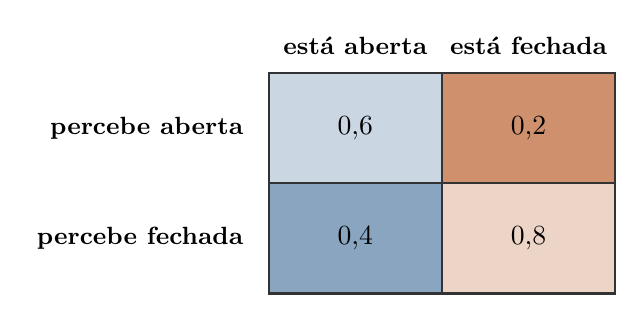
\begin{tikzpicture}[x=1cm,y=1cm]

  \def\cw{2.2}\def\ch{1.4}

  % células (fill: mais forte = mais provável)
  \fill[dblue!55]   (0,0)      rectangle (\cw,\ch);
  \fill[dorange!25] (\cw,0)    rectangle (2*\cw,\ch);
  \fill[dblue!25]   (0,\ch)    rectangle (\cw,2*\ch);
  \fill[dorange!65] (\cw,\ch)  rectangle (2*\cw,2*\ch);

  % grade
  \draw[black!80, line width=0.8pt] (0,0) grid[xstep=\cw, ystep=\ch] (2*\cw,2*\ch);
  \draw[black!80, line width=0.8pt] (0,0) rectangle (2*\cw,2*\ch);

  % valores
  \node at (0.5*\cw,1.5*\ch) {$0{,}6$};
  \node at (1.5*\cw,1.5*\ch) {$0{,}2$};
  \node at (0.5*\cw,0.5*\ch) {$0{,}4$};
  \node at (1.5*\cw,0.5*\ch) {$0{,}8$};

  % cabeçalhos de coluna
  \node[font=\small\bfseries] at (0.5*\cw,2*\ch+0.35) {está aberta};
  \node[font=\small\bfseries] at (1.5*\cw,2*\ch+0.35) {está fechada};

  % cabeçalhos de linha
  \node[font=\small\bfseries, anchor=east] at (-0.2,1.5*\ch) {percebe aberta};
  \node[font=\small\bfseries, anchor=east] at (-0.2,0.5*\ch) {percebe fechada};

\end{tikzpicture}
\end{document}
